\documentclass[oneside]{book}
\usepackage[T1]{fontenc}
\usepackage{hyperref}
\hypersetup{
  linktocpage,
  colorlinks
}
\usepackage{soul}
\usepackage{inconsolata}
\renewcommand{\familydefault}{\sfdefault}

\usepackage{graphicx}
\usepackage[dvipsnames]{xcolor}
\usepackage{pdfpages}

\definecolor{base02}{HTML}{073642}
\definecolor{base00}{HTML}{839496}
\definecolor{orange}{HTML}{b58900}
\definecolor{cyan}{HTML}{2aa198}

\usepackage{parskip}
\setlength{\parindent}{0pt}
\setlength{\parskip}{4mm}

\usepackage{listings}
\usepackage[framemethod=tikz]{mdframed}

\lstdefinelanguage{Flex}{
  otherkeywords= {\%\%, \%\{, \%\}, \%option}
}


\lstloadlanguages{C,make}
\lstset{%
showstringspaces=false,
basicstyle=\ttfamily\color{base00},
commentstyle=\ttfamily\color{red},
keywordstyle=\ttfamily\color{orange},
identifierstyle=\ttfamily\color{base00},
stringstyle=\ttfamily\color{cyan}}

\surroundwithmdframed[
  hidealllines=true,
  fontcolor=base00,
  backgroundcolor=base02,
  innerleftmargin=15pt,
  innertopmargin=15pt,
  innerrightmargin=15pt,
  roundcorner=5pt,
  innerbottommargin=5pt]{lstlisting}


\date{}

\begin{document}
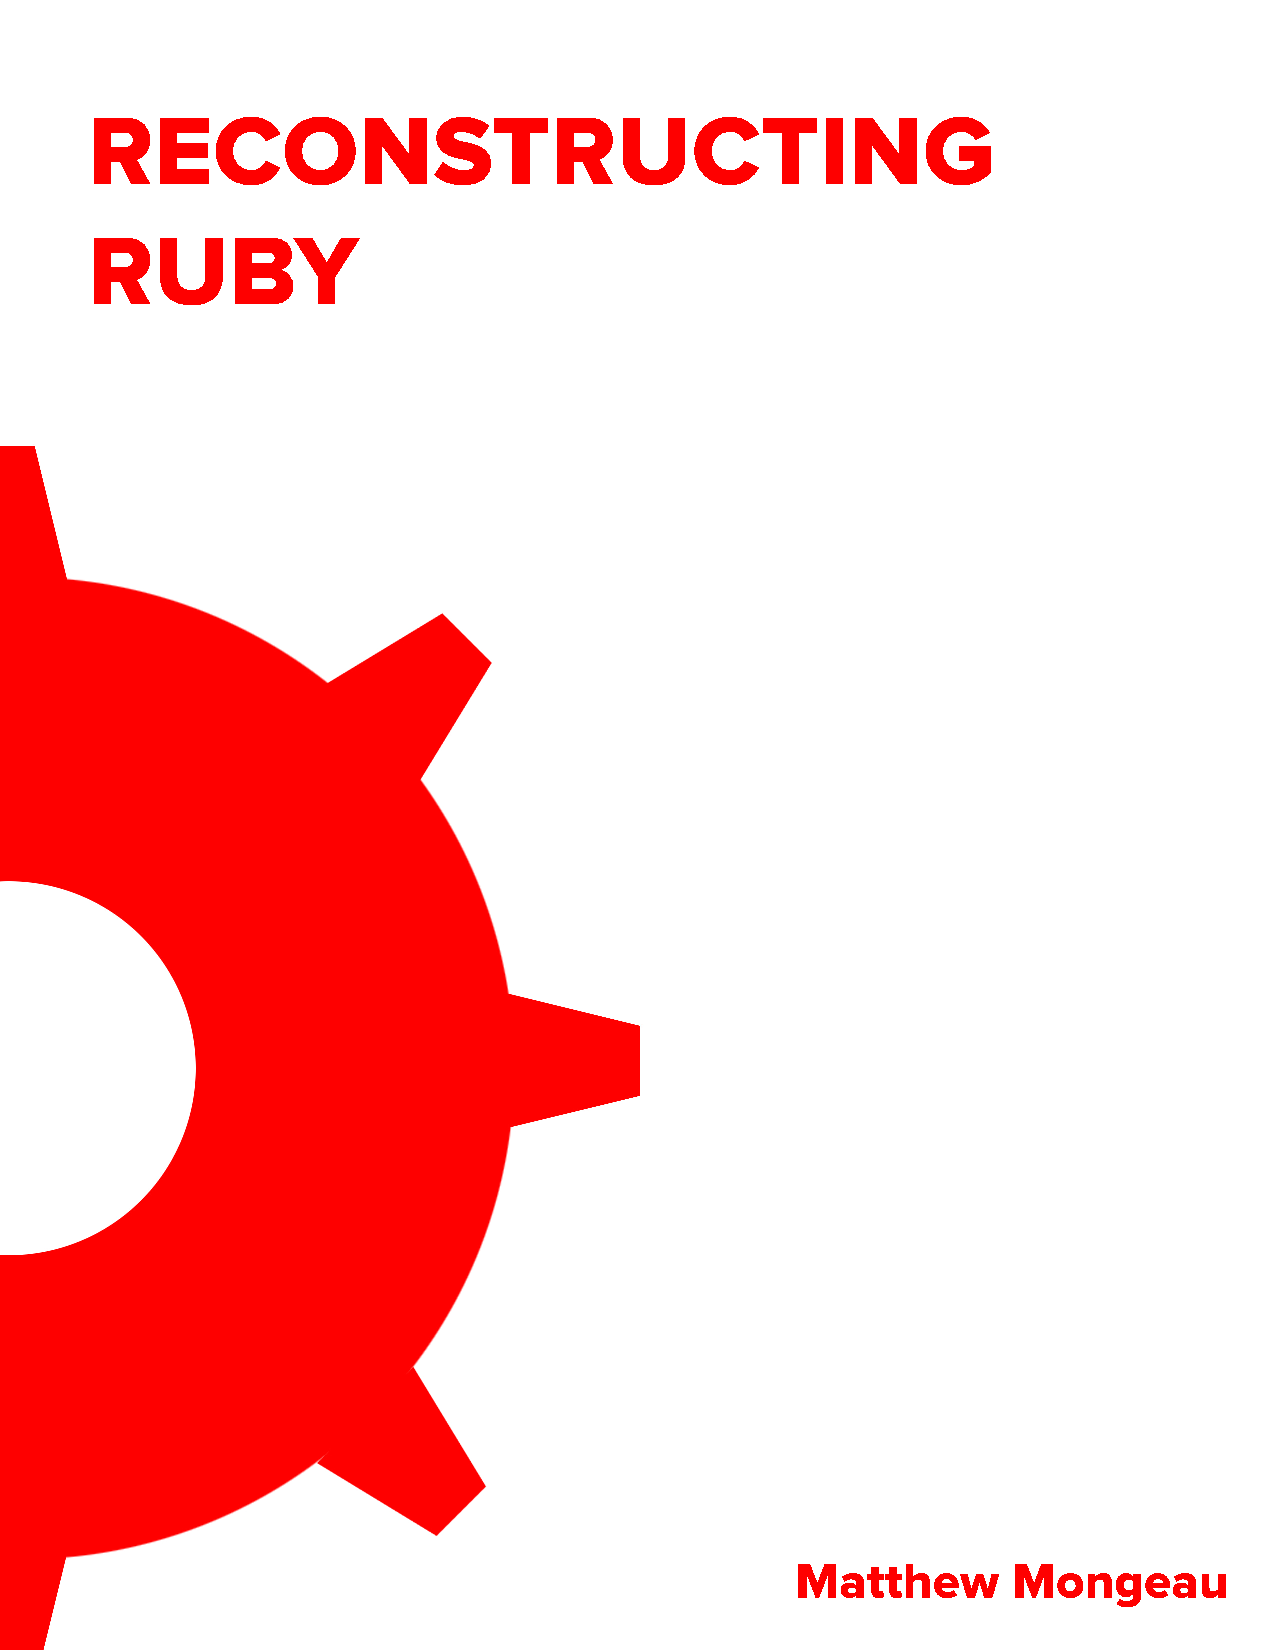
\includepdf{book/title.pdf}
\title{Reconstructing Ruby}
\author{Matthew Mongeau}
\maketitle

\frontmatter
\tableofcontents
\chapter*{Preface}

This book is not a primer on C. It assumes that you have a passing knowledge of C programming. If you've never programmed in C before it's highly suggested that you read the book "C Programming Language, 2nd Edition" by Brian W. Kernighan and Dennis M. Ritchie -  which is often referred to as "K\&R".

In addition this book expects its readers to be able to search online for terms not discussed in detail in this book.

This book has been written for two purposes. The first is to provide a better understanding of Ruby's internals, potentially allowing readers to contribute to Ruby. A second goal is to provide a better understanding of interpreters in general. The second goal opens up the possibilities for readers to create their own interpreted languages.

This book was heavily influenced by Pat Shaughnessy's "Ruby Under a Microscope".


\mainmatter
\chapter{Tokenizing}

\section{Our first lexer}

What is a lexer? The job of a lexer is to read your code and identify what we call tokens. Tokens are simply named pieces of text. We'll be using a program called Flex to tokenize our code. Flex is a lexical analyzer designed to create a tokenizer.

A Flex file will typically have this structure:

\begin{lstlisting}
definitions and directives
%%
rules
%%
user code
\end{lstlisting}

For our intents, we'll ignore adding any definitions for now. However we'll be adding a couple of directives. The first directive allows us to execute code before the lexer. This will allow us to load up some necessary C includes like stdio. It looks like:

\begin{lstlisting}[language=C]
%{
  #include <stdlib.h>
  #include <stdio.h>
%}
\end{lstlisting}

The second directive we'll add tells flex that we will not be implementing a yywrap method. yywrap is used to check if there is an additional input file to continue reading tokens from. We'll only be reading from a single file (or from the terminal) so we will just turn this off:

\begin{lstlisting}[language=C]
%option noyywrap
\end{lstlisting}

After specifying the directives, we'll follow up with some rules. The way the rules work are that they will try to match text and when it sees specific text it will execute the corresponding code. So the format for a single rule will look like:

\begin{lstlisting}[language=C]
RULE { C CODE }
\end{lstlisting}

Our first lexer is just going to recognize numbers and inform us when it has found one. Additionally we'll want to ignore anyy characters that aren't numbers so we'll need two rules:

\begin{lstlisting}[language=C]
[0-9]+ { printf("NUMBER: %s\\n", yytext); }
. {}
\end{lstlisting}

In our first rule we reference yytext. yytext is a character array that contains the text that flex has matched against. In our case it will be a character array containing some number. Each rule uses regular expression like syntax for describing what it will match. For instance, our first rule matches any number between 0 and 9 one or more times. The second rule matches any single character and executes no code on a match.

The last part of a flex file is the user code. We'll add a simple c main function to our file. This main function will call yylex which will trigger the initial flex process based on STDIN.

Let's create a file called {\bf ruby.l} and add the following content:

\begin{lstlisting}[language=Flex]
%{
  #include <stdlib.h>
  #include <stdio.h>
%}

%option noyywrap

%%
[0-9]+ { printf("NUMBER: %s\n", yytext); }
. {}
%%

int main(int argc, char *argv[]) {
  yylex();
  return EXIT_SUCCESS;
}
\end{lstlisting}

Now to compile and run this do the following

\begin{lstlisting}
flex ruby.l
cc -o ruby lex.yy.c
./ruby
\end{lstlisting}

Then try the following:

\begin{lstlisting}
1
NUMBER: 1
42
NUMBER: 42
\end{lstlisting}

Then press ctrl-c to exit

Let's simplify having to compile our ruby code by creating a Makefile. Create a file named Makefile and add the following:

\begin{lstlisting}[language=make]
all: ruby

ruby: lex.yy.c
	cc -o ruby lex.yy.c

lex.yy.c: ruby.l
	flex ruby.l

clean:
	rm ruby lex.yy.c
\end{lstlisting}

Now we can just run {\bf make} from now on when we want to compile our version of ruby. We'll modify this file as our implementation of ruby grows.

\section{Handling Files}

When writing an interpreted language we'll want the language to function in two different forms. We'll want it to work based on STDIN input as well as a file. Let's extend the lexer to operate on both. Flex defines a global input file called yyin. By default, yyin is pointing to STDIN. We can make the lexer use a file by pointing yyin to a file. Since yyin will be defined by Flex, we'll want to extern it. Let's modify the definitions and directives portion of our file to the following:

\begin{lstlisting}[language=C]
%{
  #include <stdlib.h>
  #include <stdio.h>
  extern FILE* yyin;
%}
\end{lstlisting}

Now that we can reference yyin, we'll modify our user code to point to a file. Since the user is going to execute the program like {\bf ruby program.rb} we can expect c's argv to contain the filename. Let's modify our user code to the following:

\begin{lstlisting}[language=C]
int main(int argc, char *argv[]) {
  if (argc > 1) {
    yyin = fopen(argv[1], "r");
  }
  yylex();
  return EXIT_SUCCESS;
}
\end{lstlisting}

Then create a file called {\bf program.rb} with the following:

\begin{lstlisting}
4
8
15
16
23
42
\end{lstlisting}

Now let's compile and run this program.

\begin{lstlisting}
make
./ruby program.rb 
\end{lstlisting}

\begin{lstlisting}
NUMBER: 4
NUMBER: 8
NUMBER: 15
NUMBER: 16
NUMBER: 23
NUMBER: 42
\end{lstlisting}

\section{More tokens}

Now let's add some more tokens, before we do that however let's modify our code a little with some reusable macro. Since for now we'll want to be printing the different tokens let's create a macro that makes it easy to print by modifying:

\begin{lstlisting}[language=C]
%{
  #include <stdlib.h>
  #include <stdio.h>
  extern FILE* yyin;
  #define VTYPE(str, type) printf("%s(%s)\n", str, type)
%}
\end{lstlisting}

From now one when we want to print a token we'll just use {\bf VTYPE("token type", token) }. Let's modify our rules to execute this macro when it sees a number token:


\begin{lstlisting}[language=C]
%%
[0-9]+ { VTYPE("NUMBER", yytext); }
. { fprintf(stderr, "\nUnknown token: %s\n", yytext); }
%%
\end{lstlisting}

Now when you {\bf make} and then run {\bf ./ruby program.rb} you should get the following output:

\begin{lstlisting}
NUMBER(4)

NUMBER(8)

NUMBER(15)

NUMBER(16)

NUMBER(23)

NUMBER(42)

\end{lstlisting}

Since we are now identifying number tokens let's add some more tokens. Let's change {\bf program.rb} to contain the following:

\begin{lstlisting}
x = 5
\end{lstlisting}

\chapter{Parsing}
What is parsing? Parsing is verifying the structure of our code.



\appendix
\chapter{References}

\backmatter
\chapter{Notes}
\end{document}
